% Identification of safety critical system components?
% Definition of simulation requirements & constraints
% Gamification strategy: what should the objective be, how should the user be engaged -> use the definition of Game to point this out
% Conceptual Design of Game Engine (Architecture & Features)
% Conceptual design of scenes / characters / challenges (goals, visual elements, structure)
% validation method used

\chapter{Conceptualization}\label{ch:design}
In this chapter, the game idea is presented.
All major elements of the game design process are defined and explained and requirements and constraints to the game are detailed, as well as
the structure of the framework of the game engine is described.

\section{Requirements}\label{sec:requirements}
As the major objective of the game was to create a fun environment for users to test and familiarize themselves with the topic of
aircraft system design and different architectures used, the game requirements can be defined.
\\
The game should introduce users to the concepts of redundancy and system failures, as well as different failure types such
as common-mode and common-cause failures.
The game has to have a good mix of fun and interactivity, while the sole purpose should not be entertainment, but rather a
mix of entertainment and education.
Education, in this context, is referred to as the part of awaking interest for a rather unknown topic.
Therefore, the game should be playable without any kind of knowledge regarding the topic of aircraft systems and should be easy
to get into.
Explanations and details should only be given as an addition, however should not be directly necessary to understand the basic concept
of gameplay.
It should be playable on open-door days, where it is not as pleasant to play the game only with mouse and keyboard, therefore a game pad
integration is necessary.

\section{Genre}\label{sec:genre}
The game is going to be designed as a puzzle game, where the user has different elements to build a system from.
As the game is supposed to attract interest about the topic of aircraft systems.
Puzzle games offer a way for the player to logically or conceptually solve levels, which is usually realized without
implementing any sort of time pressure~\cite{10.5555/2544002}.
That is also going to be the case in this game.

\section{Finding a name}\label{sec:finding-a-name}
The process of finding a name was lead by trying to represent both aircraft, system engineering and the puzzling aspect of the game.
A list of different names was proposed, that combine some or all of the former-mentioned elements.
The following names were available for further selection and refinement.
\begin{itemize}
    \item SkyLogic
    \item AeroSystems Architect
    \item Am I an Aircraft Systems Engineer?
    \item Aircraft Systems Engineering Puzzle
    \item Aircraft Systems Architect
\end{itemize}
The final name that was chosen for the game in order to design a logo and icon is \textit{Aircraft Systems Architect}.
Figures~\ref{fig:logo} and~\ref{fig:logo-icon} show the games' logo and icon.
\begin{figure}
    \centering
    
\includegraphics[width=\textwidth]{Pictures/res/concept/aircraft-systems-architect-logo}
    \caption{Game logo}
    \label{fig:logo}
\end{figure}
\begin{figure}
    \centering
    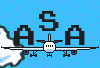
\includegraphics[width=\textwidth]{Pictures/res/concept/asa-logo}
    \caption{Game logo icon}
    \label{fig:logo-icon}
\end{figure}

\section{Game Engine Design}\label{sec:game-engine-design}
In this section, an overview of the game engine architecture and core features is given.
The design principles and development methodologies are clarified and challenges regarding the implementation will be defined.

\subsection{Architecture}\label{subsec:architecture}
The game engine uses an entity component system approach, which aims to decompose the game objects (entities) into small, reusable and interchangeable
components, that act as simple data containers to define properties of an object.
The game engine follows an object-oriented programming approach, where entities and components are designed to be easily extendable and inheritable.
This allows for an easy creation of new types of entities or components by reusing and extending existing ones, without modifying the core engine code.
To achieve this, a set of base classes for entities, components and systems is defined, which can be subclassed and implemented to provide the custom data and
properties and logics needed.
Components should simply act as data containers, which also follows the data encapsulation approach typically used in object-oriented programming, as
the interface to access the data within a component is provided by the components' getter and setter methods.
The game engine follows a modular approach, where a set of systems - which is either pre-defined by the core game engine (e.g.\ rendering, sounds) or
a custom implementation by the game - is executed by a game loop to handle inputs, game logics and updates to the entities and components.
This modular approach allows for an easy addition or removal of systems depending on the game implementation, without affecting the game loop.
This also enables for optimizations such as parallelization of the execution of the systems, which leads to performance and scalability improvements.
However, in the scope of this thesis, it may not be necessary to parallelize the game systems.

\subsection{Features}\label{subsec:features}
The core features provided by the game engine are rendering, audio handling, input handling, resource management and language management.
\\
The rendering system provides handling of different screen dimensions, options for fullscreen visualization and window mode, and allows
for rendering of different graphical objects, such as text, shapes, images or animations.
Rendering is done solely in 2D and is based on the usage of the java built-in rendering system Graphics2D, which already provides a
variety of methods to help with the rendering process.
The rendering system also provides a scaling engine, which is used to correctly detect the actual screen position against the design point (e.g.\ a
game may be developed for 1920x1080px screens, but can also be used on other screen sizes).
\\
The audio system enables the game engine to play and mix different types of sounds and music with a support for different audio formats and codecs.
It is able to handle looped audios and helps in creating and enhancing the game environment.
\\
The game engine provides a flexible input system that allows to capture a variety of user inputs, including keyboards, mouse and gamepad events.
The input system supports a customization of different key bindings to functions, as it serves as a queue of events happening during the game which
may then be processed by other systems.
\\
Resource management is a built-in feature of the game which enables the developer to easily load different file types, such as images or XML files.
This includes languages, tile sets, high score files and level files of a pre-defined format.
The resource manager may be replaced with a custom resource loader, depending on the games' needs and requirements.
\\
A major part of the game engine is the handling of text within games, as text is represented by ids which are loaded from different language files.
This enables a support for different languages within the game without having to rewrite game code.
Language files may be translated to other languages and simply included to the game, where the user may switch the language.
A language management system which is based on using IDs (tags) instead of the actual text for any text string is used.
A processor is parsing all available language files in XML format and a look-up table that maps each ID to the corresponding text string is created.
Within the Rendering Engine, each text is rendered in the language the game is set to.

\section{Game Environment Design}\label{sec:game-environment-design}
Before implementing the game itself, a concept and idea for the game was developed and a prototype was built, which was refined during the
actual implementation process of the game.
In this chapter, the process of conceptualizing and designing the game, including mechanics and gameplay, graphic concepts and
level design is explained.

\subsection{Intended Gameplay}\label{subsec:intended-gameplay}
The player is playing an aircraft mechanic, who is supposed to investigate systems for possible failures and improve the given systems or
build new systems according to given requirements.
The player is given instructions by an aircraft engineer and a tablet device with some applications to show necessary
information, requirements and tips.
There are multiple levels with advancing difficulty that may be played.
Each of these levels shows and conveys different concepts used in system engineering.
To solve the puzzle levels, the user has different components to choose from in the inventory (also called the build panel), that
can be added to the current system configuration by drag and drop.
Components can be connected by using cables and putting them in the correct places and rotations.
As the game is grid-based, there are limited possibilities which have to be considered in level design, however most levels
may be solved in different ways, which are to some degree more or less efficient.
This is represented by the score that is calculated at the end of each level after validating the systems correct functionality, which gives
a hint to the player where he or she may perform better in order to score higher.
\\
The detailed game mechanics are described in the next section~\ref{subsec:game-mechanics}.

\subsection{Game Mechanics}\label{subsec:game-mechanics}
As the general intended game play was already stated in the previous chapter, the detailed game mechanics are going to be described in this section.
In each level, a defined set of components is already available on the game grid, which may or may not be replaceable, depending on the given
information from the level file.
\\
Each component has defined simulation parameters such as failure probability and failure detection rate, which can not be changed by the user.
Another set of components is added to the users build panel in each level, where they can be placed by drag and drop to the game grid.
The goal is to use the given space on the grid efficiently and build a system that has a failure ratio below the requirement / goal target failure ratio.
Components can be connected by using different cables (red, blue, green, yellow), which simply represent different layers of cables, so multiple
cables can be placed on a single grid tile.
Cables can be rotated to correctly connect components or cables of the same type.
Each cable port type color is also shown on the component itself to make clear, which components have in- and outgoing cable ports
that cables may be connected to.
\\
After setting up the system configuration, the player can start a simulation.
This simulation calculates the markov chain of the given system and adds up the failure probability of all states that lead to a system failure with the given
input requirements.
\\
Comparing this result to the goal leads to a passed or failed level, however the distance from the players' system to the target also matters when it comes to calculating
the score, which consists of exactly this distance, the remaining components in the players inventory and a base score for each level.
During the simulation process, the aircraft starts flying through the sky to give a visualization that something is happening, as with increasing
level size the time to calculate the probabilities rises accordingly.
\\
When the level is passed successfully, a visualization of that is given by showing a score board and fireworks, when the level is failed, the aircraft
shows explosions instead.

\subsection{Graphic Design}\label{subsec:graphic-design}
The goal of the graphic design process was to conceptualize the general layout of the game environment as well as the look and feel
of the major components used.
During this process, placeholders where used in a prototype game to visualize the placement of different UI and game elements.
The graphics design process was iterative and most graphics have changed frequently throughout the game development process.
Generally, due to the requirement to keep the game relatively simple to pick up for the target audience, it was chosen to keep
the graphics design simple and clean as well.
Therefore, a classical 8-bit graphics style is chosen for all graphics of the game, including UI.
For that, a color palette of mostly bright colors and various different tones of gray is used across all graphics.
\\
The following figures show the general layout concept of the level
menu scene \ref{fig:level-menu-scene-concept} and the game scene~\ref{fig:game-scene-concept}.
\begin{figure}
    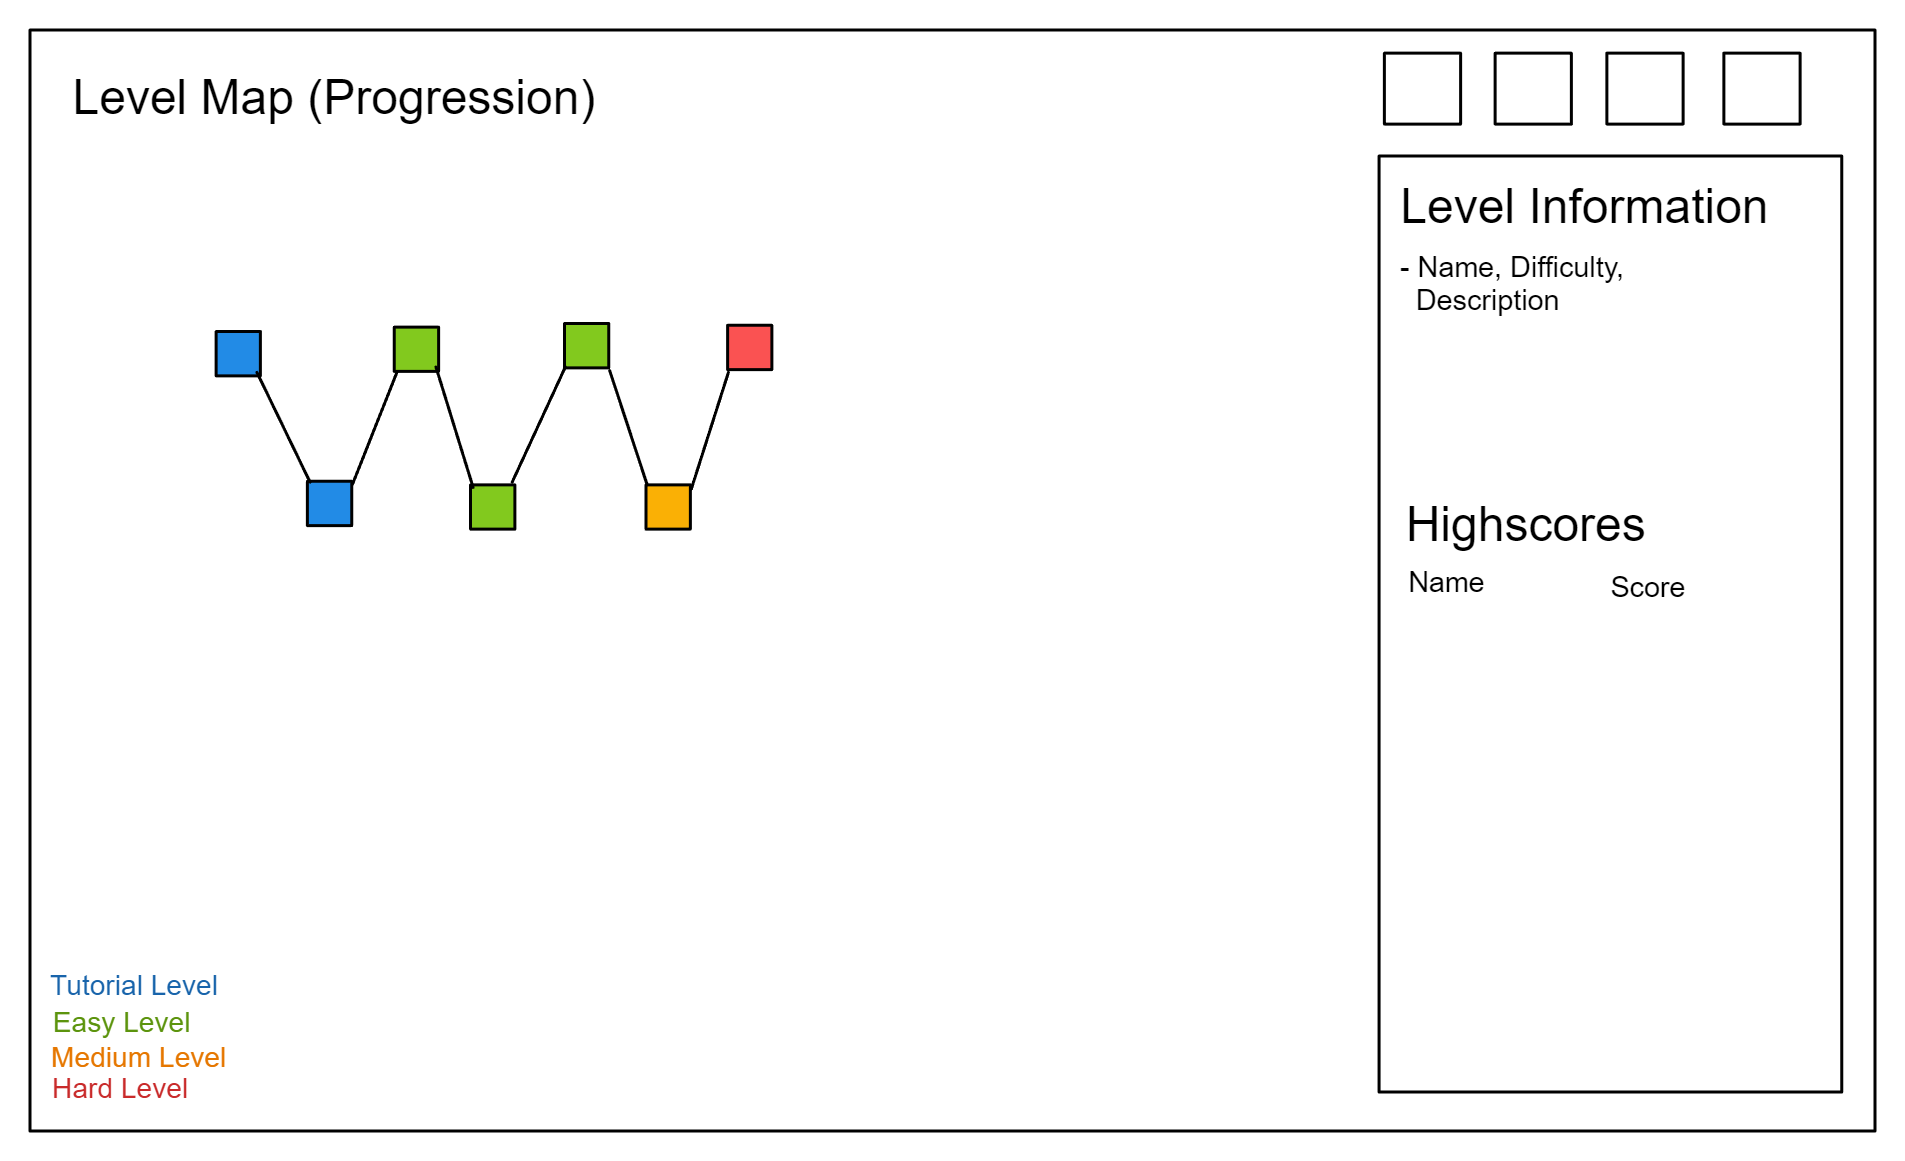
\includegraphics[width=\textwidth]{Pictures/res/concept/level-menu-scene-concept}
    \caption{Level menu scene concept}
    \label{fig:level-menu-scene-concept}
\end{figure}
\begin{figure}
    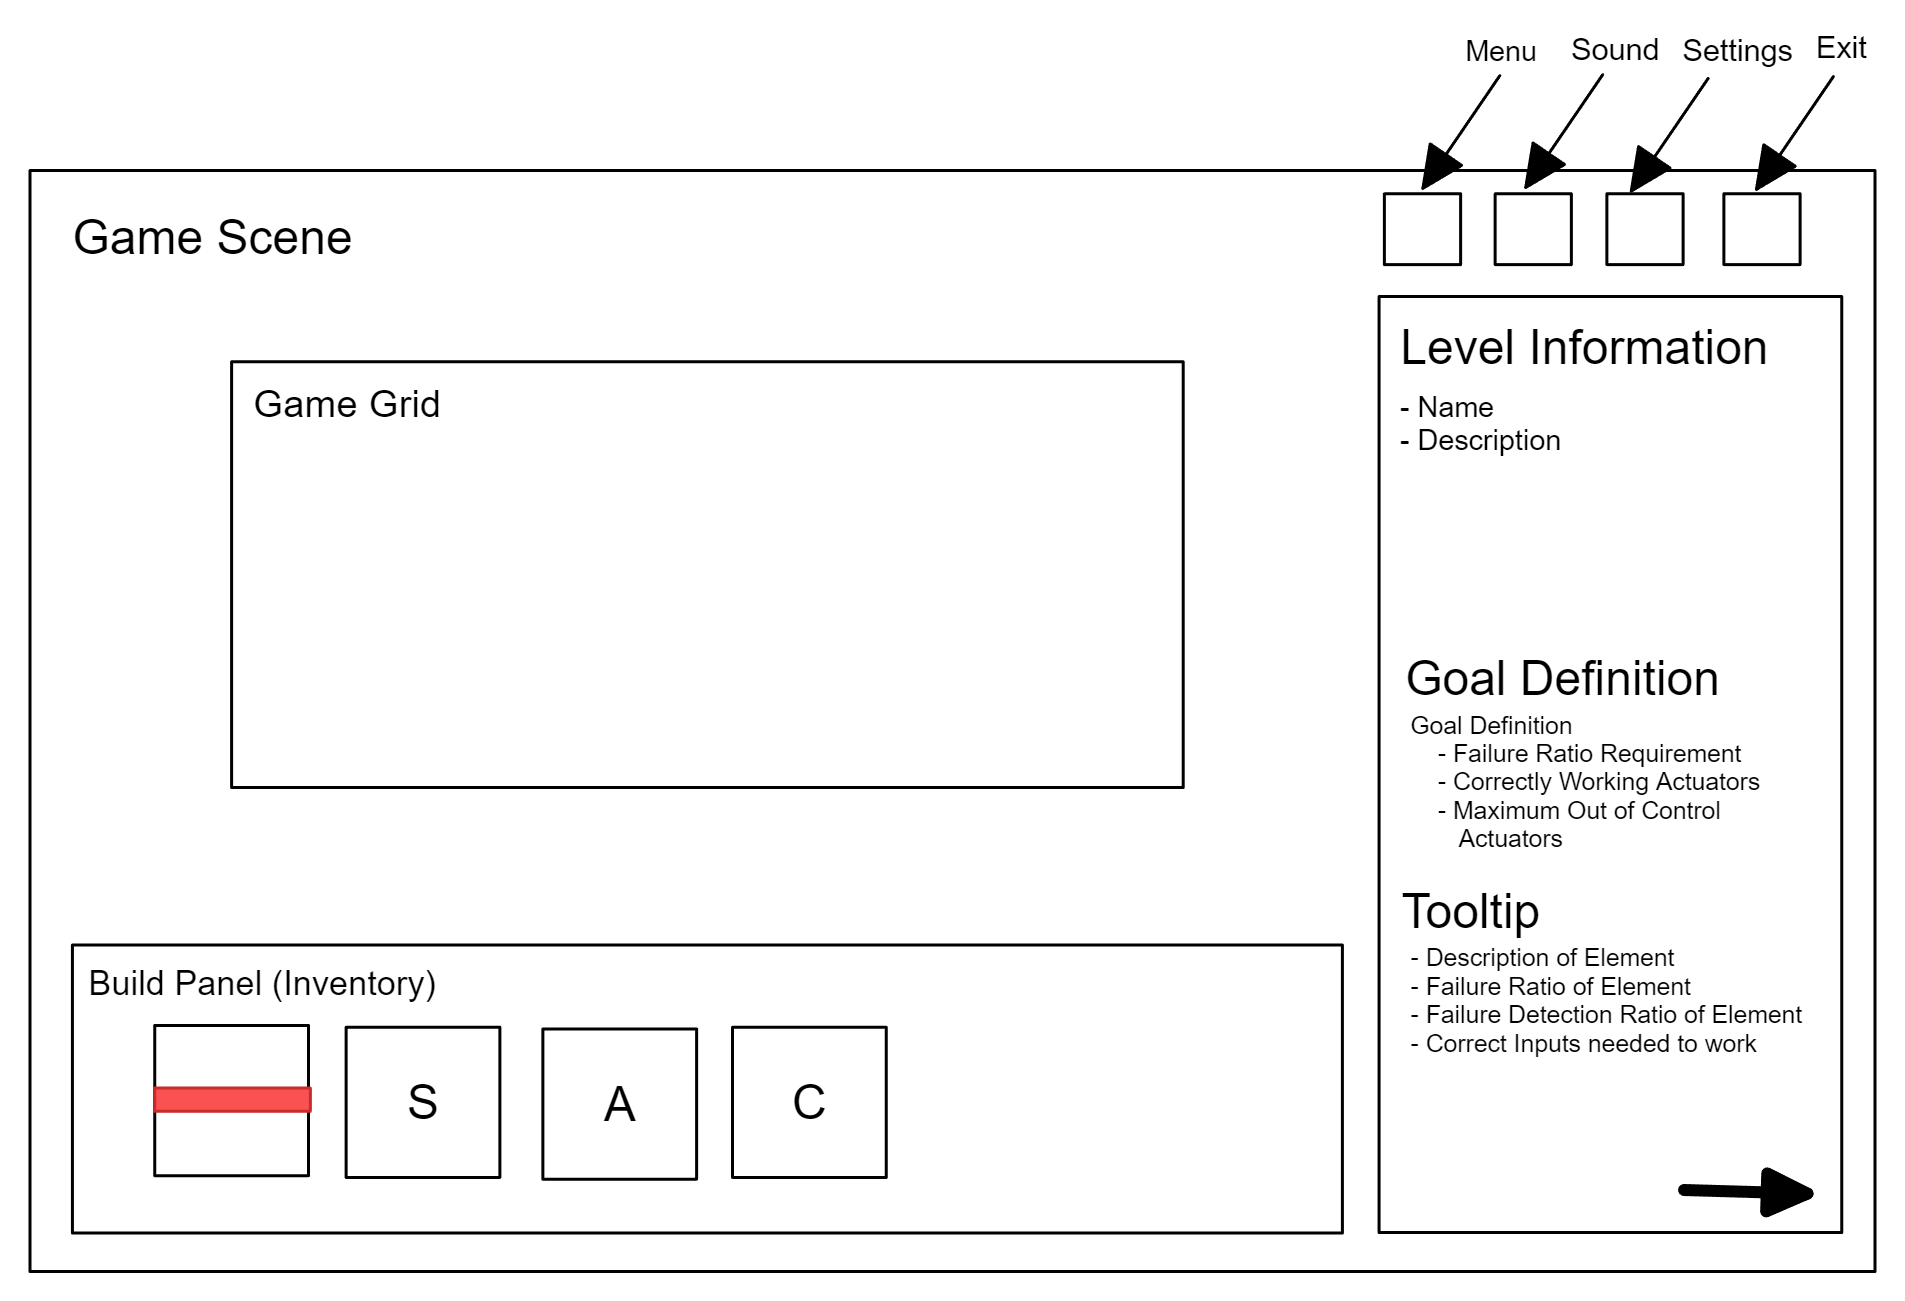
\includegraphics[width=\textwidth]{Pictures/res/concept/game-scene-concept}
    \caption{Game scene concept}
    \label{fig:game-scene-concept}
\end{figure}
According to the concept scene layouts, the following components have to be designed:
\begin{itemize}
    \item Screen backgrounds
    \item Background tiles, placeholder tiles
    \item Simulation components: actuators, sensors, computers, cables, \ldots
    \item Build panel
    \item Information panel
\end{itemize}

\subsection{Sound Design}\label{subsec:sound-design}
To provide atmosphere and create an 8 bit-styled experience, open source music will be used in the game.

\subsection{Level Design}\label{subsec:level-design}
The level design is a main part of this work, as the progression through the game and the process of explaining different concepts
within aircraft system design is heavily influenced by this.
Therefore, some levels were conceptualized before the implementation, to have a guideline for the actual implementation.
Levels are categorized in difficulties, reaching from tutorial to hard.
When passing a level, the user unlocks new levels to progress through the game, however the progression may be turned off and the user can choose from all
levels.
\\
Tutorials should guide the user through the features of this game and provide some insight on the basic gameplay and a general
understanding of aircraft systems, failures and redundancy concepts.
A visual representation of this is needed to provide enough input for younger age-groups to play and understand the game.
However, for other users, some more in-depth knowledge is also provided in order to better understand calculations, simulations and
game logic in the background.
Tutorial levels explain the basic usage, such as cable and component (re-)placement and the different safety requirement
categories.
\\
The categories are described by colors, from red (catastrophic) to blue (no safety effect).
Each component that can be built in the level also has this information to it, so the user can visually see a representation
of the criticality and the effect of the objects to the system and its requirements.
Each level goal is defined by a safety requirement and a minimum count of correctly operating actuators (or other components, such
as flight control computers, sensors, \ldots).
As the user progresses through the levels, there will be harder goals in safety requirements that need to be solved by using
redundancy concepts or mechanisms such as voting.
As this work aims to explain most of the basic concepts, some levels should also take into consideration common-mode and common-cause
failures.
\\
The following levels have been conceptualized for this game by default:
\begin{enumerate}
    \item Tutorials to explain basic game concept and system engineering concepts
    \item Duplex Systems with and without cross-strapping
    \item Triplex Systems
    \item Systems with multiple actuators
    \item Systems with duplex sensors
    \item Common-Mode Failure scenario
    \item Common-Cause Failure scenario
\end{enumerate}
Each level has a defined goal, that has to be achieved in order to pass the level.
Tutorials aim to explain the basic concepts of gameplay and systems, such as placing components, connecting and rotating cables and
explaining the difference between out of control and passive failures, failure probability, failure detection ratio / integrity and the purpose
of different components that may be used to complete the levels.
\\
During the conceptualization, high-level designs for each level, including layouts, objectives and possible additional content were created.
Sketches and visualizations of the level ideas helped to create a baseline for the implementation that was used later during development of the levels.
During the implementation and production process of the game, most of the level designs were revised and adjustments were made, which is also
an iterative task where updates may be needed in the future.
\\
The finalized level designs and implementations will be shown in section~\ref{subsec:level-implementation}.
\\
Additionally, through a build mode the user is able to set up new levels including the requirements / level goal via the built-in
frontend, which then saves the level to a new xml file.

\subsection{Tutorials}\label{subsec:tutorials}
As some text is necessary to correctly explain the gameplay and concepts such as redundancy, characters are designed in order to create
a dialogue with the player to make the experience, even though reading is an essential part of the game, more user-friendly and interactive.
The characters available to the game, which appear whenever dialogues and tutorials should be shown, are the character representing the user, who is displayed
as an aircraft mechanic who has to repair and investigate different systems in the aircraft and another character who gives the user instructions and
leads the user through the game, who is an aircraft systems engineer.

\subsection{Language}\label{subsec:language}
As the game is supposed to be used by a broad audience, especially in Germany and at the University Day of the University of Stuttgart, there should be an option
to change the language.
Therefore, english, german and a simplified version of the german text file are supported by default.